\documentclass[border=2pt]{standalone}
\usepackage{amsmath}
\usepackage{tikz}
\usetikzlibrary{matrix}

\begin{document}

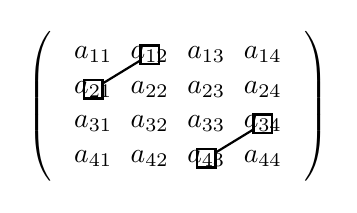
\begin{tikzpicture}
  \matrix (m) [matrix of math nodes,left delimiter=(,right delimiter=)] {
    a_{11} & a_{12} & a_{13} & a_{14} \\
    a_{21} & a_{22} & a_{23} & a_{24} \\
    a_{31} & a_{32} & a_{33} & a_{34} \\
    a_{41} & a_{42} & a_{43} & a_{44} \\
  };

  % Define a style for consistent circles and lines
  \tikzset{
    mycircle/.style={draw, thick, black},
    myline/.style={thick, black}
  }

  % Draw circles around specific elements
  \node[mycircle] (c12) at (m-1-2.center) {};
  \node[mycircle] (c21) at (m-2-1.center) {};
  \node[mycircle] (c34) at (m-3-4.center) {};
  \node[mycircle] (c43) at (m-4-3.center) {};

  % Draw lines connecting the circles
  \draw[myline] (c21) -- (c12);
  \draw[myline] (c43) -- (c34);

\end{tikzpicture}

\end{document}
